\section{Slu\v cajevi upotrebe}

Ve\' c smo objasnili pojam slu\v cajeva upotrebe i dijagram slu\v cajeva upotrebe u opisu kori\v s\' cenih tehnika. Ono \v sto nismo rekli jeste da svaki slu\v caj upotrebe mora da bude pra\' cen svojim opisom.\\

Opis slu\v caja upotrebe bi trebalo da bude dovoljno duga\v cak, tj. da obuhvati sve ono \v sto je potrebno da bi neko mogao na osnovu tog opisa da napravi ta\v cnu implementaciju. Dobar opis slu\v caja upotrebe sadr\v zi dovoljno informacija da se mo\v ze sagledati kada, kako, ko i sa kojim podacima u\v cestvuje u slu\v caju upotrebe (\cite{smalkov-slajdovi}).\\

U skladu sa time, opisi slu\v cajeva upotrebe u ovom radu obuhvataju slede\'ce:
\begin{itemize}
	\item naziv (slu\v zi za jedinstveno identifikovanje slu\v caja upotrebe u sistemu), 
	\item u\v cesnike (korisnici koji u\v cestvuju u slu\v caju upotrebe),
	\item preduslove (zahtevi i uslovi koji moraju biti ispunjeni pre samog po\v cetka slu\v caja upotrebe), 
	\item postuslove (zahtevi i uslovi koji moraju biti ispunjeni nakon samog zavr\v setka slu\v caja upotrebe), 
	\item glavni tok (numerisana lista koraka koji \v cine scenario slu\v caja upotrebe), 
	\item alternativne tokove (scenarija do kojih dolazi pri odstupanju nekog od koraka glavnog toka), i 
	\item dodatne formulare od zna\v caja.
\end{itemize}

\subsection{Prijava na evidenciju}

Nezaposleno lice dolazi li\v cno u Nacionalnu slu\v zbu za zapo\v sljavanje radi prijave na evidenciju. U zavisnosti od toga da li je lice ve\' c bilo na evidenciji ili ne razlikujemo dva slu\v caja:

\begin{itemize}
	\item ukoliko lice nije bilo nikada ranije prijavljeno na evideniciji, izvr\v sava se slu\v caj upotrebe Prva prijava (\ref{su: prva prijava})
	\item ukoliko je lice bilo prijavljeno na evidenciju ali je izgubilo status aktivnog tra\v zenja posla zbog neredovnog javljanja izvr\v sava se slu\v caj upotrebe Ponovna prijava (\ref{su: ponovna prijava}).
\end{itemize}

\begin{figure}[H]
	\centering
	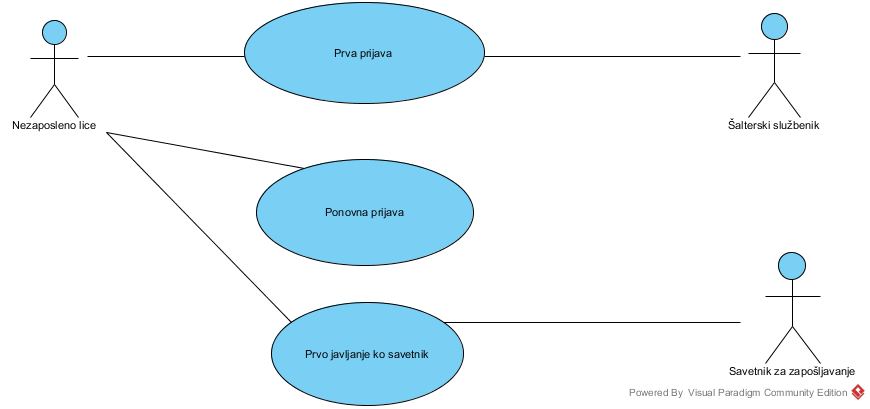
\includegraphics[width=0.8\textwidth]{dijagrami/dijagrami-slucajeva-upotrebe/prijava-na-evidenciju.png}
	\caption{Dijagram slu\v cajeva upotrebe procesa "Prijava na evidenciju"}
	\label{dsu: prijava na evidenciju}
\end{figure}

\subsubsection{Slu\v caj upotrebe: Prva prijava}
\label{su: prva prijava}

\noindent U\v cesnici: Nezaposleno lice (u daljem tekstu NL), \v salterski slu\v zbenik (u daljem tekstu \v SS)
\\
\\ Preduslovi: NL ima li\v cnu kartu i dokaz o stru\v cnoj spremi. Automat za izdavanje broja je u funkciji. \v SS je ulogovan na sistem. 
\\
\\ Postuslovi: NL je ili uspe\v sno prijavljen na evidenciju i izdat je evidencioni karton tra\v zioca zaposlenja, ili mu je ukazano na njegov status.
\\
\\ Glavni tok:
\begin{enumerate}
	\item NL prilazi automatu i bira opciju ''Prijava na evidenciju''.
	\item Automat bele\v zi da je opcija ''Prijava na evidenciju'' odabrana, ra\v cuna naredni broj u redu \v cekanja za tu opciju, i \v stampa papir sa brojem.
	\item NL uzima broj i \v ceka svoj red.
	\item Kada do\dj e na red, NL prilazi \v salteru i zahteva od \v SS da ga prijavi na evidenciju.
	\item \v SS otvara formular za prijavu.
	\item \v SS tra\v zi od NL da mu preda li\v cnu kartu i dokaz o stru\v cnoj spremi.
	\item NL predaje potrebna dokumenta. 
	\item \v SS popunjava formular na osnovu predatih dokumenata.
	\item \v SS daje NL-u da popuni Obrazac za prijavu na evidenciju.
	\item NL popunjava Obrazac za prijavu na evidenciju, a zatim ga vra\' ca \v SS-u.
	\item \v SS popunjava Evidencioni karton za tra\v zioca zaposlenja.
	\item \v SS zakazuje prvo javljanje savetniku za zapo\v sljavanje, i postavlja status NL-a na ''aktivan''.
	\item \v SS vra\' ca dokumenta NL-u i daje mu evidentacioni karton.
	\item Prelazi se na slu\v caj upotrebe \ref{su: prvo javljanje savetniku}.
\end{enumerate}

\noindent Alternativni tokovi: 
\begin{description}
	\item[A1. Pad sistema] ~\\
	Ukoliko se u bilo kom koraku Glavnog toka dogodi pad sistema na kojem radi \v SS, \v SS ponovo pokre\'ce sistem i prijavljuje se na njega.
	\begin{enumerate}
		\item \v SS proverava da li je formular sa\v cuvan.
		\item Ukoliko jeste, prelazi se na korak 9 Glavnog toka.
		\item Ina\v ce, prelazi se na korak 8 Glavnog toka.
	\end{enumerate}

	\item[A2. Status NL-a je ''zamrznut''] ~\\
	Ukoliko u koraku 8 Glavnog toka sistem prika\v ze da postoje informacije o NL-u, kao i da je njegov status ''zamrznut'', \v SS menja njegov status u ''aktivan''. Izvr\v savanje se nastavlja u koraku 11 Glavnog toka.
\end{description}

\subsubsection{Slu\v caj upotrebe: Ponovna prijava}
\label{su: ponovna prijava}

\noindent  U\v cesnici: Nezaposleno lice (u daljem tekstu NL), \v salterski slu\v zbenik (u daljem tekstu \v SS)
\\
\\ Preduslovi: NL ima li\v cnu kartu. Automat za izdavanje broja je u funkciji. \v SS je ulogovan na sistem. 
\\
\\ Postuslovi: NL-u je uspe\v sno promenjen status i izdat je novi evidencioni karton tra\v zioca zaposlenja.
\\
\\ Glavni tok:
\begin{enumerate}
	\item NL prilazi automatu i bira opciju ''Prijava na evidenciju''.
	\item Automat bele\v zi da je opcija ''Prijava na evidenciju'' odabrana, ra\v cuna naredni broj u redu \v cekanja za tu opciju, i \v stampa papir sa brojem.
	\item NL uzima broj i \v ceka svoj red.
	\item Kada do\dj e na red, NL prilazi \v salteru i zahteva od \v SS da mu promeni status.
	\item \v SS tra\v zi od NL da mu preda li\v cnu kartu.
	\item NL predaje li\v cnu kartu.
	\item \v SS pronalazi NL-a u sistemu. 
	\item \v SS bira opciju izmeni podatke.
	\item \v SS menja status "zamrznut" u "aktivan".
	\item \v SS popunjava Evidencioni karton za tra\v zioca zaposlenja.
	\item \v SS zakazuje prvo javljanje savetniku za zapo\v sljavanje, i postavlja status NL-a na ''aktivan''.
	\item \v SS vra\' ca dokumenta NL-u i daje mu evidentacioni karton.
	\item Prelazi se na slu\v caj upotrebe \ref{su: prvo javljanje savetniku}.
\end{enumerate}

\noindent Alternativni tok: /

\subsubsection{Slu\v caj upotrebe: Prvo javljanje savetniku}
\label{su: prvo javljanje savetniku}

\noindent U\v cesnici: Nezaposleno lice (u daljem tekstu NL), savetnik za zapo\v sljavanje (SZ)
\\
\\ Preduslovi: NL ima evidentacioni karton. SZ je ulogovan na sistem. 
\\
\\ Postuslovi: Ili je uspe\v sno zabele\v zeno javljanje NL-a ili je postavljen status NL-a na ''zamrznut''.
\\ 
\\ Glavni tok:
\begin{enumerate}
	\item NL dolazi kod SZ-a u kancelariju i predaje mu svoj evidentacioni karton.
	\item SZ pronalazi NL-a u sistemu.
	\item SZ i NL razgovaraju o NL-ovoj stru\v cnoj spremi, kakvi poslovi zanimaju NL-e, i koje ve\v stine Nl poseduje.
	\item SZ unosi nove informacije u sistem.
	\item SZ tra\v zi informacije o prethodnim zaposlenjima NL-a, i ako postoje i te informacije, SZ ih unosi u sistem.
	\item SZ zakazuje slede\' ce javljanje i vra\' ca NL-u evidentacioni karton.
\end{enumerate}

\noindent Alternativni tok:
\begin{description}
	\item[A1. Promena statusa NL-a na ''zamrznut''] ~\\
	Ukoliko u koraku 1 Glavnog toka NL ne do\dj e na prvo javljanje pre zakazanog termina, automatski se \v salje zahtev za izmenom podataka o NL-u u sistemu, i to: status NL-a se prebacuje na ''zamrznut''. Slu\v caj upotrebe se zavr\v sava.
\end{description}


\begin{mylandscape}
	\subsubsection{BPMN dijagrami}
	
	\begin{figure}[H]
		\centering
		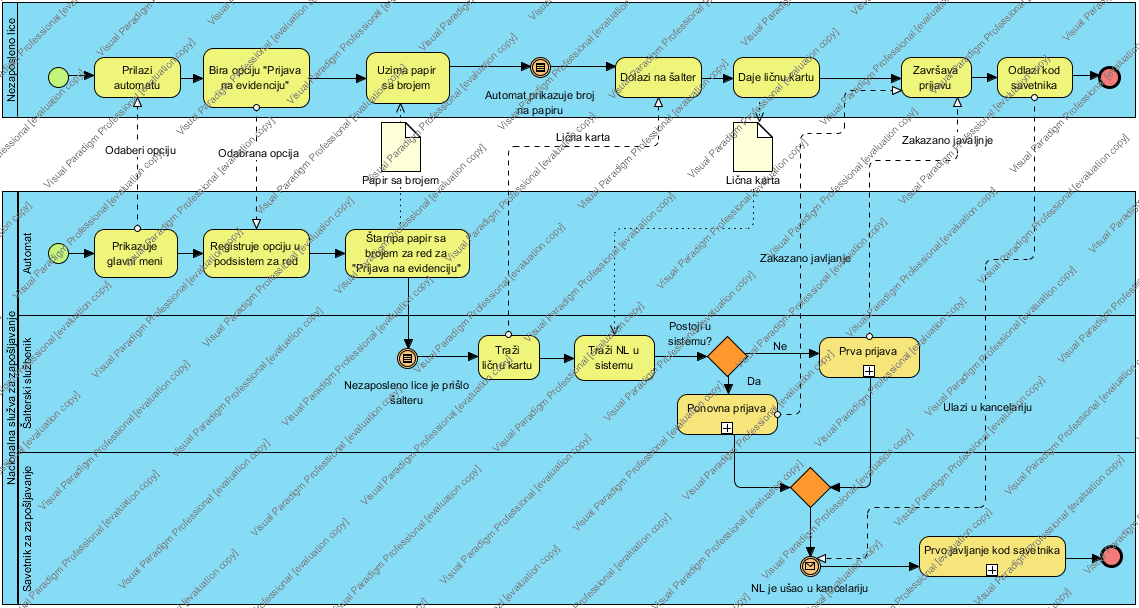
\includegraphics[width=0.6\paperwidth]{dijagrami/bpmn-dijagrami/prijava-na-evidenciju.png}
		\caption{BPMN dijagram procesa ''Prijava na evidenciju''.}
		\label{bpmnd: prijava na evidenciju}
	\end{figure}
	
	\newpage
	
	\begin{figure}[H]
		\centering
		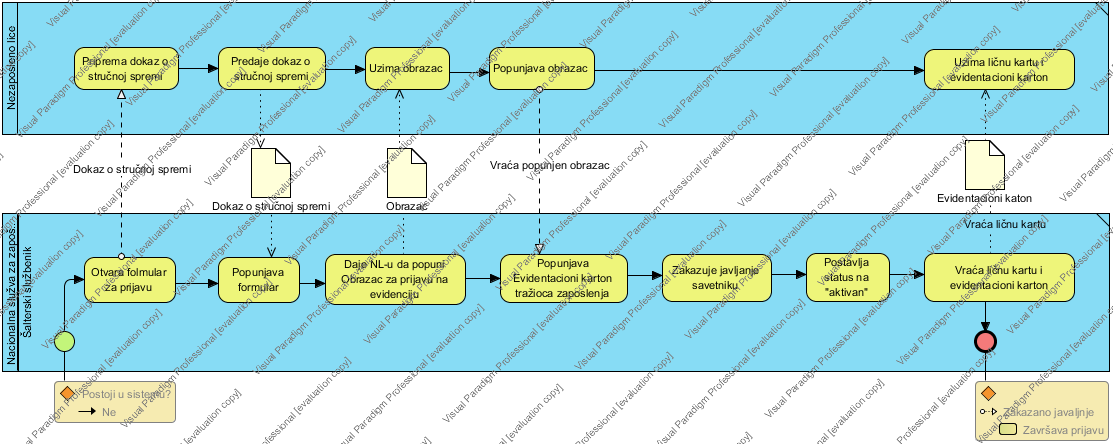
\includegraphics[width=0.8\paperwidth]{dijagrami/bpmn-dijagrami/prva-prijava.png}
		\caption{BPMN dijagram potprocesa ''Prva prijava'' procesa ''Prijava na evidenciju'' (Slika \ref{bpmnd: prijava na evidenciju}).}
	\end{figure}
	
	\newpage
	
	\begin{figure}[H]
		\centering
		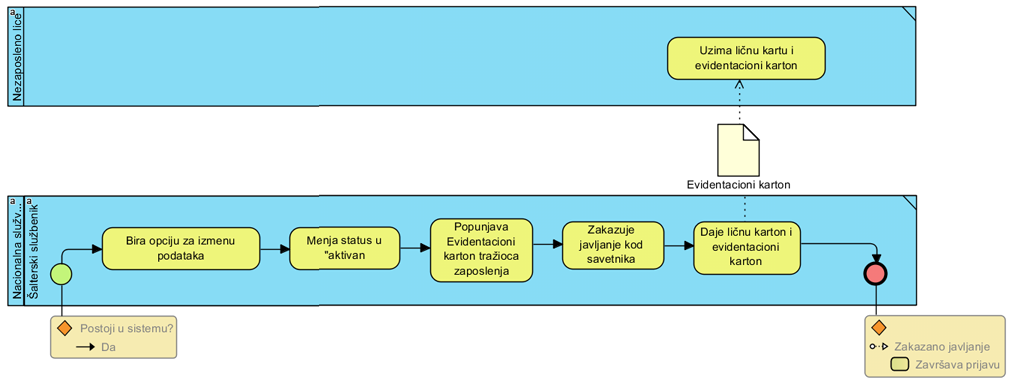
\includegraphics[width=0.8\paperwidth]{dijagrami/bpmn-dijagrami/ponovna-prijava.png}
		\caption{BPMN dijagram potprocesa ''Ponovna prijava'' procesa ''Prijava na evidenciju''  (Slika \ref{bpmnd: prijava na evidenciju}).}
	\end{figure}
	
	\newpage
	
	\begin{figure}[H]
		\centering
		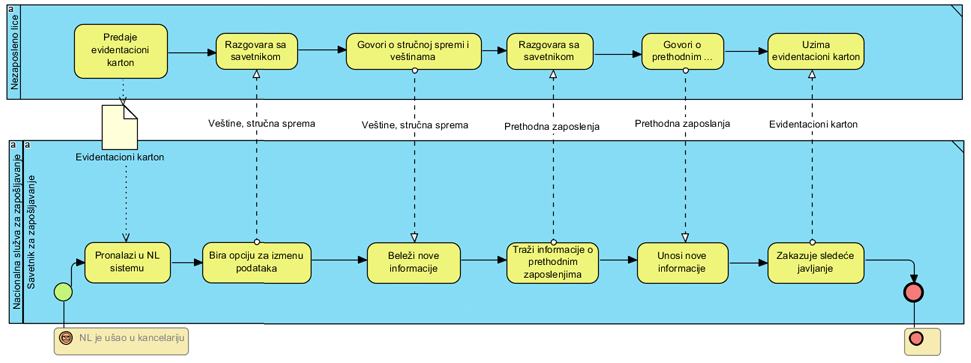
\includegraphics[width=0.8\paperwidth]{dijagrami/bpmn-dijagrami/prvo-javljanje-kod-savetnika.png}
		\caption{BPMN dijagram potprocesa ''Prvo javljanje savetniku'' procesa ''Prijava na evidenciju''  (Slika \ref{bpmnd: prijava na evidenciju}).}
	\end{figure}
\end{mylandscape}